\section{\textbf{Evaluation Measures}}
To evaluate our proposed system we used several statistical measures such as Confusion matrix, Precision, Recall, F$_1$ score and graphical measures such as Precision-Recall curve, Receiver Operating Characteristics (ROC) curve.
\subsection{\textbf{Confusion Matrix}}
A confusion matrix is a table that is used to evaluate the performance of a classification model. As ours is a binary classification model, the confusion matrix of our system has two rows and two columns. This matrix reports the number of false positives, false negatives, true positives, and true negatives.
\par
\vspace{0.3cm}
\noindent
\textbf{Fig.} \ref{fig:CM} shows confusion matrix for our system.\clearpage
\begin{figure}[h!]
    \centering
    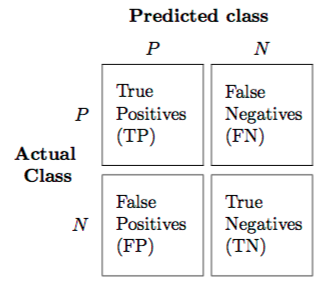
\includegraphics[scale=0.50]{Figures/confusion_matrix_1.png}
    \caption{Confusion Matrix}
    \label{fig:CM}
\end{figure}
\begin{itemize}
    \item True Positive(TP): Number of documents that is suspicious and also classified as suspicious.\vspace{0.2cm}
    \item True Negative(TN): Number of documents that is non suspicious and also classified as non suspicious.\vspace{0.2cm}
    \item False Negative(FN): Number of documents that is suspicious but classified as non suspicious.\vspace{0.2cm}
    \item False Positive(FP): Number of documents that is non suspicious but classified as suspicious. 
\end{itemize}
\noindent
This numbers are used to calculate other evaluation measures.

\subsection{\textbf{Precision}}
Precision refers as positive predictive value. That is the ratio of correctly classified positive instances to the total number of instances classified as positive. Precision can be obtained form  the following equation.
\begin{equation}
    \texttt{Precision} = \frac{TP}{TP+FP}
\end{equation}
If precision is high then the algorithm is doing well.

\subsection{\textbf{Recall}}
Recall is the ratio of correctly classified positive instances to the total number of positive instances. It is also called true positive rate. Recall can be obtained from the following equation.
\begin{equation}
    \texttt{Recall} = \frac{TP}{TP+FN}
\end{equation}
High precision and high Recall is essential for a model.

\subsection{\textbf{$F_1$ score}}
 $F_1$ score is the weighted average of Precision and Recall. To chose a learning algorithm between several algorithms we have to find $F_1$ Score of algorithms. F1-score can be obtained from the following equation,
 \begin{equation}
     F_1 = \frac{2*precision*recall}{precision+recall}
 \end{equation}
$F_1$ score is usually more useful than accuracy

\subsection{\textbf{Precision Recall Curve}}
Precision Recall curves summarize the trade-off between the true positive rate and the positive predictive value for a predictive model using different probability thresholds. A precision-recall curve is a plot of the precision (y-axis) and the recall (x-axis) for different thresholds.

\subsection{\textbf{ROC Curve}}
Receiver Operating Characteristic (ROC) curves summarize the trade-off between the true positive rate and false positive rate for a predictive model using different probability thresholds.%ROC curves are appropriate when the observations are balanced between each class. 
It is a plot of the false positive rate (x-axis) versus the true positive rate (y-axis) for a number of different candidate threshold values between 0 and 1.